\documentclass[12pt]{article}
% Load packages
\usepackage{url}  % Formatting web addresses
\usepackage{ifthen}  % Conditional
\usepackage{multicol}   %Columns
\usepackage[utf8]{inputenc} %unicode support
\usepackage{amsmath}
\usepackage{amssymb}
\usepackage{epsfig}
\usepackage{epstopdf}
\usepackage{graphicx}
\usepackage[margin=0.1pt,font=footnotesize,labelfont=bf]{caption}
\usepackage{setspace}
%\usepackage{longtable}
\usepackage{colortbl}
%\usepackage{palatino,lettrine}
%\usepackage{times}
%\usepackage[applemac]{inputenc} %applemac support if unicode package fails
%\usepackage[latin1]{inputenc} %UNIX support if unicode package fails
\usepackage[wide]{sidecap}
%\usepackage[authoryear,round,comma,sort&compress]{natbib}
\usepackage[square,sort,comma,numbers,sort&compress]{natbib}
%\usepackage[authoryear,round]{natbib}
\usepackage{supertabular}
\usepackage{simplemargins}
\usepackage{fullpage}
\usepackage{comment}
\usepackage{lineno}
%\usepackage{chicago}
\usepackage{textcomp}
\usepackage{multirow}
\usepackage{amsmath}
\usepackage[linesnumbered,lined,boxed,commentsnumbered]{algorithm2e}
\DeclareMathOperator*{\argmin}{\arg\!\min}

\usepackage{algorithm2e}
\usepackage{algpseudocode}
%\usepackage[space]{cite}
\urlstyle{rm}

%\textwidth = 6.50 in
%\textheight = 9.5 in
%\oddsidemargin =  0.0 in
%\evensidemargin = 0.0 in
%\topmargin = -0.50 in
%\headheight = 0.0 in
%\headsep = 0.25 in
%\parskip = 0.15in
%\linespread{1.75}
\doublespace

%\bibliographystyle{chicago}
\bibliographystyle{plos2009}

\makeatletter
\renewcommand\subsection{\@startsection
	{subsection}{2}{0mm}
	{-0.05in}
	{-0.5\baselineskip}
	{\normalfont\normalsize\bfseries}}
\renewcommand\subsubsection{\@startsection
	{subsubsection}{2}{0mm}
	{-0.05in}
	{-0.5\baselineskip}
	{\normalfont\normalsize\itshape}}
\renewcommand\section{\@startsection
	{subsection}{2}{0mm}
	{-0.2in}
	{0.05\baselineskip}
	{\normalfont\large\bfseries}}
\renewcommand\paragraph{\@startsection
	{paragraph}{2}{0mm}
	{-0.05in}
	{-0.5\baselineskip}
	{\normalfont\normalsize\itshape}}
\makeatother

%Review style settings
%\newenvironment{bmcformat}{\begin{raggedright}\baselineskip20pt\sloppy\setboolean{publ}{false}}{\end{raggedright}\baselineskip20pt\sloppy}

%Publication style settings

% Single space'd bib -
\setlength\bibsep{0pt}

\renewcommand{\rmdefault}{phv}\renewcommand{\sfdefault}{phv}
\newcommand{\norm}[1]{\left\lVert#1\right\rVert}

% Change the number format in the ref list -
\renewcommand{\bibnumfmt}[1]{#1.}

% Change Figure to Fig.
\renewcommand{\figurename}{Fig.}

% Begin ...
\begin{document}
\begin{titlepage}
{\par\centering\textbf{\Large {Reduced order modeling and analysis of the human complement subsystem}}}
\vspace{0.05in}
{\par \centering \large{Adithya Sagar, Wei Dai$^{\#}$, Mason Minot$^{\#}$, and Jeffrey D. Varner$^{*}$}}
\vspace{0.10in}
{\par \centering {School of Chemical and Biomolecular Engineering}}
{\par \centering {Cornell University, Ithaca NY 14853}}
\vspace{0.1in}
{\par \centering \textbf{Running Title:}~Reduced order model of complement}
\vspace{0.1in}
{\par \centering \textbf{To be submitted:}~\emph{PLoS~ONE}}
\vspace{0.5in}
{\par \centering $^{\#}$ Denotes equal contribution}
\vspace{0.1in}
{\par \centering $^{*}$Corresponding author:}
{\par \centering Jeffrey D. Varner,}
{\par \centering Professor, School of Chemical and Biomolecular Engineering,}
{\par \centering 244 Olin Hall, Cornell University, Ithaca NY, 14853}
{\par \centering Email: jdv27@cornell.edu}
{\par \centering Phone: (607) 255 - 4258}
{\par \centering Fax: (607) 255 - 9166}
\end{titlepage}
\date{}
\thispagestyle{empty}
\pagebreak
%%%%%%%%%%%%%%%%%%%%%%%%%%%%%%%%%%%%%%%%%%%%%%%%%%%%%%%%%%%%%%%%%%%%%%%%%%%%%%%%%%%%%%%%%%%%%%%%%%%%%%%%%%%
%%%%%%%%%%%%%%%%%%%%%%%%%%%%%%%%%%%%%%%%%%%%%%%%%%%%%%%%%%%%%%%%%%%%%%%%%%%%%%%%%%%%%%%%%%%%%%%%%%%%%%%%%%%
\section*{Abstract}
Complement is a central part of innate immunity and plays a very significant role in regulating the inflammatory response.
In this study, we present an effective biochemical network modeling approach in building a reduced order model to study a complex biochemical network, the human complement system. The key innovation of our approach is the use of simple equations to capture the behavior of a complex biochemical network.  We developed a hybrid modeling approach which combines ODEs and logical rules to model biochemical processes for which a complete mechanistic understanding is missing. Using this modeling framework we  incorporated computational simulation and experimental validation of the lectin and alternative pathway to examine C3 and C5 convertase formation and activity. The reduced order model consisted of only 18 differential equations with 28 kinetic and control parameters. Thus, the model was several orders of magnitude smaller and includes more pathways than comparable purely ODE models in the literature. We estimated the model parameters from in vitro human complement time-course experiments of C3a and C5a from Morad and coworkers \cite{morad2015time}, in the presence and absence of zymosan, and without the classical pathway. We then compared the model predictions with C3a and C5a data sets, for alternative and lectin pathway dynamics, that were not used for model training. Once validated, we performed sensitivity analysis on the model to estimate which parameters were critical to model performance in several conditions. The reduced order hybrid approach produced a surprisingly predictive human complement model, much similar to the study on human coagulation using the same modeling framework \cite{sagar2015dynamic}. Taken together, the combined analysis of alternate and lectin pathways along with the incorporation of the downstream reactions involving C5 convertase elucidated new insight into roles of governing parameters that mediate the complement system. Deeply understanding how the main governing parameters change with respective to the different combinations of pathway activation will greatly aid in development of drugs for strategic therapeutic targets. Due to the low computational cost relative to the existing models and accuracy of our predictions, we believe that our reduced order complement network is the first step towards building a computation toolbox for treatment analysis or clinical screening in the medical field.

%We further tested the predictive power of the coagulation model parameters against data not used in training, and found good agreement between simulations and experimental measurements. Lastly, we tested the performance of DOPS on commonly used test functions for global optimization and on published biochemical parameter estimation benchmark problems. For the wide range of problems that we considered, DOPS outperformed other meta-heuristic approaches despite a limited number of function evaluations.

\vspace{0.1in}
{\noindent \textbf{Keywords:}~Biochemical engineering, systems biology, reduced order models, complement system}

% Extra abstract
% Mathematical modeling of biological systems with multiple feed back loops is one such area where parameter estimation is a difficult non-linear optimization problem. This difficulty is further compounded when dealing with parameter vectors of high dimensions.

%In this study, we present the dynamically dimensioned particle
%a novel meta-heuristic approach that combines a variant of particle swarm optimization (PSO) along with dynamically dimensioned search (DDS) to obtain near optimal solutions of high dimensional biochemical networks within a relatively few function evaluations.
%We use a particle swarm optimization technique that uses multi-swarms to generate candidate vectors which are then greedily updated using DDS by dynamically varying the perturbed parameter dimensions. We tested this algorithm (25 trials with 4000 function evaluations in each trial) on a biochemical network of coagulation (148 parameters and 92 species) and compared it's performance against other meta-heuristics like Differential Evolution (DE), Particle Swarm Optimization (PSO), Simulated Annealing (SA) and also against DDS alone. The new algorithm outperforms all the other meta-heuristics on the coagulation model. The parameter vectors obtained using this approach fit the experimental data well and also make accurate enough predictions on unseen experimental data. We also performed this comparison on commonly used test functions (Ackley and Rosenbrock) for global optimization and found the same behavior. Further we used two recently published benchmark problems, a genome wide kinetic model with 1759 parameters and a metabolic model of Chinese Hamster Ovary cells with 117 parameters to evaluate the performance of our approach. We  surprisingly performed well on these benchmarks and obtained the nominal parameter vector with just 4000 function evaluations in both cases.

\pagebreak

\setcounter{page}{1}

% Uncomment in production -
\linenumbers


\section*{Introduction}
Complement is a central part of innate immunity and plays a very significant role in regulating the inflammatory response. Complement was first discovered in the 1890s where it was found to 'complement' the bactericidal activity of natural antibodies. Complement is mediated through a set of approximately 30-35 soluble and cell surface proteases. The central process in complement activation involves the formation of Membrane Attack Complex (MAC) and a protein called C5a. C5a acts as a bridge between innate and adaptive immunity and plays a very important role in regulating inflammation and coagulation.  Complement activation takes places through three different pathways: the alternate, the classical and the lectin. Each of these pathways involves a different initiator signal that leads to the formation of a serine protease called C5 convertase which cleaves an inactive protein called C5 to form C5a and C5b. The classical pathway is triggered when antibodies form complexes with foreign antigens or other pathogens. A multimeric protein complex C1 binds to the antigen-antibody complex and undergoes a conformational change. This activated complex cleaves proteins C4 and C2 to C4a, C4b, C2a and C2b respectively. C4a and C2b combine to form a protease C4bC2a also known as the classical C3 convertase. The lectin pathway is initiated through the binding of L-ficolin or Mannose Binding Lectin (MBL) to the carbohydrates on the surfaces of bacterial pathogens. This bound complex in turn cleaves C4 and C2 and leads to the production of C4bC2a. The alternate pathway involves a 'tickover' mechanism in which a protein called C3 is hydrolyzed to form C3b. In presence of foreign pathogens C3b binds to these surfaces and recruits  additional factors called factor B and factor D that lead to the formation of alternate C3 convertase - C3bBb. The formation of classical and alternate C3 convertases on bacterial surfaces is followed by the formation of proteases called C5 convertases. The classical and alternate C3 convertases recruit C3, Factor B and Factor D to form classical C5 convertase (C4bC2aC3b) and alternate C5 convertase (C3bBbc3B) respectively. The C5 convertases then cleave C5 to form C5a and C5b respectively. 	The cleavage of C5 is followed by a series of sequential cleavages of proteins C6, C7, C8 and C9 that combine with C5b to form the MAC complex.

The activation of complement and formation of C5a and MAC complex is regulated at different points through a number of plasma and host cell proteins.
The initiation of the classical pathway through the attachment of C1 to an antibody is controlled by the C1 Inhibitor (C1-Inh), a protease inhibitor belonging to the serpin superfamily. C1-Inh irreversibly binds to and deactivates the active subunits of component C1 to prevent spontaneous fluid phase and chronic activation of complement \cite{walker1995complement}. The serum and host-tissue regulation of the upstream elements of the complement system is also achieved through the binding of C4 binding protein (C4BP) to C4b and through the binding of factor H to C3b \cite{blom2001structural}. These proteins are also capable of binding their respective components in the convertase form. Membrane cofactor protein (MCP or CD46) possesses a cofactor activity for C4b and C3b, which protects the host from self-activation of complement \cite{riley2004cd46}.  Delay accelerating factor (DAF or CD55) is able to recognize and dissociate both convertases \cite{lukacik2004complement}. MAC is inhibited by vitronectin and clusterin in the plasma and CD59 at the host surface.
Proteins C3a, C4a, and C5a are inactivated or reduced in activity by carboxypeptidase-N \cite{liszewski1995control}.

Given the complexity and importance, developing mathematical models of complement are crucial to understanding its dynamics. Complement models have typically been formulated as linear or non-linear Ordinary Differential Equation (ODE) systems. Hirayama  et al. (ref) used a system of linear ODEs to model the classical pathway of complement. Korotaevskiy and co-workers (ref) built a theoretical model of complement using a system of non-linear ODEs that included classical, lectin and alternate pathways. However both these studies involve no validation studies with experimental data. Liu et al used analyzed the formation of classical and lectin C3 convertases and the regulatory role of C4BP using a system of 45 non-linear ODEs with 85 parameters.  Recently, Zewde and co-workers built a detailed mechanistic model of alternative complement activation was built using 107 ODEs and 74 kinetic parameters (Ref). This model delineated the response of complement on a host cell and a foreign antigen. However, these previous models were largely based upon mechanistic knowledge.  However given the complexity of complement and its interactions with other networks like coagulation, autonomous nervous system, adaptive immunity it is unfeasible and computationally expensive to build such large mechanistic models. In addition is much more difficult to experimentally interrogate the response of various complement proteins under different conditions. This also presents with the problem of estimation of a large number of parameters with little or no experimental data. Thus there exists a need to reduce the mechanistic complexity while capturing dynamics of complement accurately.

In this study, we present an effective biochemical network modeling approach in building a reduced order model to study a complex biochemical network, the human complement system. The key innovation of our approach is the use of simple equations to capture the behavior of a complex biochemical network.  We developed a hybrid modeling approach which combines ODEs and logical rules to model biochemical processes for which a complete mechanistic understanding is missing. Using this modeling framework we  incorporated computational simulation and experimental validation of the lectin and alternative pathway to examine C3 and C5 convertase formation and activity. The reduced order model consisted of only 18 differential equations with 28 kinetic and control parameters. Thus, the model was several orders of magnitude smaller and includes more pathways than comparable purely ODE models in the literature. We estimated the model parameters from in vitro human complement time-course experiments of C3a and C5a from Morad and coworkers \cite{morad2015time}, in the presence and absence of zymosan, and without the classical pathway. We then compared the model predictions with C3a and C5a data sets, for alternative and lectin pathway dynamics, that were not used for model training. Once validated, we performed sensitivity analysis on the model to estimate which parameters were critical to model performance in several conditions. The reduced order hybrid approach produced a surprisingly predictive human complement model, much similar to the study on human coagulation using the same modeling framework \cite{sagar2015dynamic}. Taken together, the combined analysis of alternate and lectin pathways along with the incorporation of the downstream reactions involving C5 convertase elucidated new insight into roles of governing parameters that mediate the complement system. Deeply understanding how the main governing parameters change with respective to the different combinations of pathway activation will greatly aid in development of drugs for strategic therapeutic targets. Due to the low computational cost relative to the existing models and accuracy of our predictions, we believe that our reduced order complement network is the first step towards building a computation toolbox for treatment analysis or clinical screening in the medical field.

\clearpage

\section*{Results}

\subsection*{Formulation of a reduced order complement model}
We developed a reduced order human complement network consisting of the most crucial steps of the human complement system (Fig. \ref{fig-schematic}). The core of our model was based upon the experimental measurements of Morad and coworker's earlier work \cite{morad2015time}, we only consider the activation of complement system through the alternate and the lectin pathways. In doing so we aim to capture a complex biological phenomenon using a few simple ordinary differential equations.  A trigger event initiates the lectin pathway in the presence of zymosan, which activates the cleavage of C2 and C4 into C2a and C2b, and C4a and C4b respectively. Classical Pathway (CP) C3 convertase (C4aC2b) is a combination of C4a and C2b, which catalyzes the cleavage of C3 into C3a and C3b. Similarly, the activation of the alternative pathways happens through the spontaneous hydrolysis of C3 which facilitates the cleavage of C3. C3b then could combine with with C3 to form alternate pathway (AP) C3 convertase. Both C3 convertases catalyze the cleavage of C3 into C3a and C3b, and C3b can then combine with either CP or AP C3 convertase to form C5 convertase, CP or AP respectively that is responsible for the cleavage of C5 to C5a and C5b. Lectin pathway activation was approximated using a combination of saturation kinetics and Hill-like function control functions. These control coefficients then modified the rates of model processes at each time step. Hill-like transfer functions $0 \le \mathbf{f (Z)}  \le 1$ quantified the contribution of components upon a target process, in this study, $\mathbf{Z}$ represents the abundance of the initiator. Taken together, while the reduced order human complement model encodes significant biological complexity, it is highly compact (consisting of only 18 differential equations). Thus, it will serve as an excellent proof of principle example to study the reduction of a highly complex human subsystem.

\subsection*{An ensemble of complement models was estimated using dynamically dimensioned search.}
A critical challenge for any dynamic model is the estimation of kinetic parameters. We estimated
kinetic and control parameters in a hierarchical fashion using  two $in~vitro$ time-series human complement data sets with and without zymosan present. The residual between simulation and experimental measurements were minimized  using dynamically dimensioned search (DDS). An initial parameter set was initialized with randomized kinetic and control parameters and allowed to search for parameter vectors that minimized the residual. Knowing that the kinetic and control parameters of the lectin pathway does not affect the dynamics of the alternate pathway, we used a hierarchal approach that estimated the parameters for the alternative pathway and lectin pathway separately. For the alternative pathway, we utilized the time-course experimental measurements of Morad and coworkers \cite{morad2015time} of $C3a$ and $C5a$ in the absence of zymosan and only allowed the alternative parameters to vary (Fig. \ref{fig-fit} A and B). The estimated alternate parameters was then fixed for the determination of lectin pathway parameters. The training for the lectin parameters, we used the experimental measurements of $C3a$ and $C5a$ in the presence of $1$ g of zymosan published by Morad et al \cite{morad2015time} (Fig. \ref{fig-fit} C and D).
The reduced human complement model captured the behavior of the alternative and lectin pathways through the time-course abundance of C3a and C5a (Fig. \ref{fig-fit}).
However we were not able to capture the curvature of the C5a alternative (Fig. \ref{fig-fit}).
The decreasing slope of the experimental measurements may be an indication of the decreasing cofactors that are required for the spontaneous hydrolysis in the alternative pathway, which we neglected.  Taken together, the model identification results suggested that our reduced order approach could reproduce a panel of lectin pathway initiation data sets in the neighborhood of physiological factor and inhibitor concentrations. However, it was unclear whether the reduced order model could predict new data, without updating the model parameters.

We tested the predictive power of the reduced order human complement model with validation data sets not used during model training. Six validation data sets were used, three for $C3a$ and $C5a$ respectively at different zymosan concentrations. All kinetic and control parameters were
fixed for the validation simulations.
The reduced order model predicted the $C3a$ and $C5a$ time-course profiles at a qualitative level (Fig. \ref{fig-prediction}).

\subsection*{Global Sensitivity analysis of the reduced order complement model}
We conducted a Sobol's sensitivity analysis to estimate which parameters controlled the performance of the reduced order model. We calculated the sensitivity of the change in $C3a$ and $C5a$ profiles using the residuals between simulation and experimentally measured data for the cases of $0$ and $1 g$ zymosan (Fig. \ref{fig-SA}. For the cases in absence of zymosan where only the alternative pathway is active, we observed that only a few variables are responsible for the system response. For $C3a$ alternate, the sensitivity analysis found that $k_{c3b~basal}$ and $k_{degradationC3a}$ are the only sensitive parameters. This gives us new insight in which of the parameters play a role in complement activation. Even though $AP~C3~Convertase$ is also responsible in the conversion of $C3$ and the production of $C3a$, the kinetic parameters that govern the equation was not sensitive at all. This elucidated that the activation of alternative pathway is more heavily governed by the spontaneous hydrolysis of $C3$ rather than the activity of $AP~C3~Convertase$. Surprisingly, closely examining the sensitive parameters that control $C5a$, in addition to the expected kinetic and control parameters related to the formation of $AP~C5~Convertase$, we observed that $k_C3~Convertase2$, the was previously not sensitive to $C3a$, to be sensitive in the formation of $C5a$. The $AP~C3~Convertase$ is a substrate required for the formation of $AP~C5~Convertase$ and the formation of $C3b$. The change in activity of $AP C3 Convertase$  will not drastically change the $C3a$ dynamics, but will effect $AP~C5a~Convertase$ formation and $C5a$ formation. The our reduced order human complement model in combination with Sobol's sensitivity analysis was able to unravel important indirect parameter interaction.

Our sensitivity analysis yielded expected results for the lectin pathway analyzes (Fig. \ref{fig-SA} (C and D)). One key difference that was observed between the sensitivity of the parameters between $C3a$ an $C5a$ was their respective degradation terms. The degradation constant of $C3a$ was sensitive between the two different cases of zymosan that was tested while the degradation constant of the $C5a$ was not sensitive. We believe this different is attributed to the magnitude of the parameters and their respective concentrations.


\clearpage

%As the dimensionality of  increases, the search region gets widened and thus the problem becomes more challenging.
%

\section*{Discussion}

The discussion has three (sometimes four) paragraphs:
\begin{enumerate}
	\item{\textbf{First~paragraph}: Present a modified version of the last paragraph of the introduction. In this study, [...]. Taken together, [killer statement]}
	\item{\textbf{Second~paragraph}: Contrast the key findings of the study with other computational/experimental studies}
	\item{\textbf{Third~paragraph}: Present future directions. If you had more time, what would like to do? Highlight the key shortcomings of the approach and how will we address them in the future.
	In this case, we will have a scaling issue if we extend to genome scale. We should extend to dynamic cases, and we need to experimentally validate the findings. }
\end{enumerate}

In this study, we present an effective biochemical network modeling approach in building a reduced order model to study a complex biochemical network, the human complement system. The key innovation of our approach is the use of simple equations to capture the behavior of a complex biochemical network.  We developed a hybrid modeling approach which combines ODEs and logical rules to model biochemical processes for which a complete mechanistic understanding is missing. Using this modeling framework we  incorporated computational simulation and experimental validation of the lectin and alternative pathway to examine C3 and C5 convertase formation and activity. The reduced order model consisted of only 18 differential equations with 28 kinetic and control parameters. Thus, the model was several orders of magnitude smaller and includes more pathways than comparable purely ODE models in the literature. We estimated the model parameters from in vitro human complement time-course experiments of C3a and C5a from Morad and coworkers \cite{morad2015time}, in the presence and absence of zymosan, and without the classical pathway. We then compared the model predictions with C3a and C5a data sets, for alternative and lectin pathway dynamics, that were not used for model training. Once validated, we performed sensitivity analysis on the model to estimate which parameters were critical to model performance in several conditions. The reduced order hybrid approach produced a surprisingly predictive human complement model, much similar to the study on human coagulation using the same modeling framework \cite{sagar2015dynamic}. Taken together, the combined analysis of alternate and lectin pathways along with the incorporation of the downstream reactions involving C5 convertase elucidated new insight into roles of governing parameters that mediate the complement system. Deeply understanding how the main governing parameters change with respective to the different combinations of pathway activation will greatly aid in development of drugs for strategic therapeutic targets. Due to the low computational cost relative to the existing models and accuracy of our predictions, we believe that our reduced order complement network is the first step towards building a computation toolbox for treatment analysis or clinical screening in the medical field.

The performance of the reduced order complement model was impressive given its limited size. However, there are several critical questions that should be explored following this study. A logical progression for this work would include expanding the network to include the classical pathway and the formation of the membrane attack complex (MAC). It is unclear whether the addition of the classical pathway will decrease the prediction of our existing model due to the cross-talk between the classical and lectin activation shown by Liu et al \cite{liu2011computational}. One potential approach in addressing such difficulties would be the incorporation of additional species such as C reactive proteins (CRP) and L-ficolin (LF) that involved in complement initiation of classical and lectin pathways. The influence of CRP, LF and the cross-talk can be captured through additional control functions that act upon the initiation pathways in a logical integration rule developed by Wayman and coworkers \cite{wayman2015dynamic}. Another issue with our reduced order model involve the omitted species that are implicitly lumped together with our effective kinetics and control parameters. Due to the reduction of parameters, the model cannot determine the dynamics or explicit impact of the omitted species on the system. However, we have created a hierarchy approach for parameter estimation that can be used to uncouple the kinetic parameter and contribution of any additional complement proteins and regulators. Using this simple and versatile modeling approach that we created, we took the first step in the development of a computation toolkit that can be readily used in a clinical setting. Our reduced order complement model is computationally inexpensive, and versatile so it could easily be incorporated into pre-existing or new pharmacokinetic models. Furthermore this approach model has the potential to create individualized treatment plans for patients with complement deficiency.

\clearpage

\section*{Materials and Methods}
We used ordinary differential equations (ODEs) to model the time evolution of proteins ($x_{i}$) in our reduced order complement model:
\begin{equation}
	\frac{dx_{i}}{dt}  =  \sum_{j = 1}^{\mathcal{R}}\sigma_{ij}r_{j}\left(\mathbf{x},\mathbf{\epsilon},\mathbf{k}\right)\qquad{i=1,2,\hdots,\mathcal{M}}\\
\end{equation}
where $\mathcal{R}$ denotes the number of reactions, $\mathcal{M}$ denotes the number of protein species in the model.
The quantity $r_{j}\left(\mathbf{x},\mathbf{\epsilon},\mathbf{k}\right)$ denotes the rate of reaction $j$.
Typically, reaction $j$ is a non-linear function of biochemical species abundance, as well as unknown kinetic parameters $\mathbf{k}$ ($\mathcal{K}\times{1}$).
The quantity $\sigma_{ij}$ denotes the stoichiometric coefficient for species $i$ in reaction $j$.
If $\sigma_{ij}>0$, species $i$ is produced by reaction $j$.
Conversely, if $\sigma_{ij}<0$, species $i$ is consumed by reaction $j$, while $\sigma_{ij} = 0$ indicates species $i$ is not connected with reaction $j$.
Species balances were subject to the initial conditions $\mathbf{x}\left(t_{o}\right) = \mathbf{x}_{o}$.

The reaction rate was written as the product of a kinetic term ($\bar{r}_{j}$) and a control term ($v_{j}$), $r_{j}\left(\mathbf{x},\mathbf{k}\right) = \bar{r}_{j}v_{j}$.
In this study, we used either saturation or mass action kinetics.
The control term $0\leq v_{j}\leq 1$ depended upon the combination of factors which influenced rate process $j$.
For each rate, we used a rule-based approach to select from competing control factors.
If rate j was influenced by $1,\dots,m$ factors, we modeled this relationship as
$v_{j} = \mathcal{I}_{j}\left(f_{1j}\left(\cdot\right),\hdots,f_{mj}\left(\cdot\right)\right)$
where $0\leq f_{ij}\left(\cdot\right)\leq 1$ denotes a regulatory transfer function quantifying the influence of factor $i$ on rate $j$.
The function $\mathcal{I}_{j}\left(\cdot\right)$ is an integration rule which maps the output of regulatory transfer functions into a control
variable. Each regulatory transfer function took the form:
\begin{equation}\label{eqn:control-factor}
	f_{ij}\left(\mathcal{Z}_{i},k_{ij},\eta_{ij}\right) = k_{ij}^{\eta_{ij}}\mathcal{Z}_{i}^{\eta_{ij}}/\left({1 + k_{ij}^{\eta_{ij}}\mathcal{Z}_{i}^{\eta_{ij}}}\right)
\end{equation}where $\mathcal{Z}_{i}$ denotes the abundance factor $i$, $k_{ij}$ denotes a gain parameter, and $\eta_{ij}$ denotes a cooperativity parameter.
In this study, we used $\mathcal{I}_{j}\in\left\{\max,\min\right\}$ \cite{pr3010138}. If a process has no modifying factors, $v_{j} = 1$.

We used saturation kinetics to model the lectin pathway activation and C3 and C5 convertase activity $\bar{r}_{j}$:
\begin{equation}\label{eqn:rate-saturation}
	\bar{r}_{j} = k_{j}^{max}\epsilon_{i}\left(\frac{x_{s}^{\eta}}{K_{js}^{\eta} + x_{s}^{\eta}}\right)
\end{equation}
where $k_{j}^{max}$ denotes the maximum rate for reaction $j$, $\epsilon_{i}$ denotes the enzyme abundance which catalyzes reaction $j$, $\eta$ denotes a cooperativity parameter (similar to a Hill coefficient), and $K_{js}$ denotes the saturation constant for species $s$ in reaction $j$. On the other hand,
we used mass action kinetics to model the protein conversion reactions within the network $\bar{r}_{j}$:
\begin{equation}\label{eqn:rate-action}
	\bar{r}_{j} = k_{j}^{max}\epsilon_{i}\prod_{s\in{m_{j}^{-}}}x_{s}
\end{equation}
where $k_{j}^{max}$ denotes the maximum rate for reaction $j$, $\epsilon_{i}$ denotes the enzyme abundance which catalyzes reaction $j$. The product in Eqn \eqref{eqn:rate-action} was carried out over the set of \textit{reactants} for reaction $j$ (denoted as $m_{j}^{-}$).


\subsection*{Estimation of an ensemble of model parameters.}
Model parameters were estimated by minimizing the difference between simulations and experimental C3a and C5a measurements (squared residual):
\begin{equation}\label{eqn:objective-function}
	\min_{\mathbf{k}} \sum_{\tau=1}^{\mathcal{T}}\sum_{j=1}^{\mathcal{S}}\left(\frac{\hat{x}_{j}\left(\tau\right) - x_{j}\left(\tau,\mathbf{k}\right)}{\omega_{j}\left(\tau\right)}\right)^{2}
\end{equation}where $\hat{x}_{j}\left(\tau\right)$ denotes the measured value of species $j$ at time $\tau$, $x_{j}\left(\tau,\mathbf{k}\right)$ denotes the simulated
value for species $j$ at time $\tau$, and $\omega_{j}\left(\tau\right)$ denotes the experimental measurement variance for species $j$ at time $\tau$. The outer summation is with respect to
time, while the inner summation is with respect to state. We minimized the model residual using Particle swarm optimization (PSO) \citep{PSO}.
PSO uses a \textit{swarming} metaheuristic to explore parameter spaces.
A strength of PSO is its ability to find the global minimum, even in the presence of potentially many local minima, by communicating the local
error landscape experienced by each particle collectively to the swarm. Thus, PSO acts both as a local and a global search algorithm.
For each iteration, particles in the swarm compute their local error by evaluating the model equations using their specific parameter vector realization.
From each of these local points, a globally best error is identified. Both the local and global error
are then used to update the parameter estimates of each particle using the rules:
\begin{eqnarray}
	\mathbf{\Delta}_{i} &=&\theta_{1}\mathbf{\Delta}_{i} + \theta_{2}\mathbf{r}_{1}\left(\mathcal{L}_{i} - \mathbf{k}_{i}\right) + \theta_{3}\mathbf{r}_{2}\left(\mathcal{G} - \mathbf{k}_{i}\right) \\
	\mathbf{k}_{i} &=& \mathbf{k}_{i} + \mathbf{\Delta}_{i}
\end{eqnarray}where $\left(\theta_{1},\theta_{2},\theta_{3}\right)$ are adjustable parameters, $\mathcal{L}_{i}$ denotes the local best solution found by particle $i$, and
$\mathcal{G}$ denotes the best solution found over the entire population of particles. The quantities $r_{1}$ and $r_{2}$ denote uniform random vectors with the same dimension as the number of unknown model
parameters \linebreak($\mathcal{K}\times{1}$). In thus study, we used $\left(\theta_{1},\theta_{2},\theta_{3}\right) = \left(1.0, 0.05564, 0.02886\right)$. The quality of parameter
estimates was measured using goodness of fit (model residual). The particle swarm optimization routine was implemented in the Python programming language.
All plots were made using the Matplotlib module of Python \citep{Matplotlib}.
%The optimization and plotting code can be downloaded from http://www.varnerlab.org.
%Experimental data,simulation code,parameter ensembles and initial conditions for each experimental simulation can be viewed and downloaded from https://github.com/jeffreyvarner/HybridCoagulationModel\_v1.


\subsection*{Global sensitivity analysis of model performance}
We conducted a global sensitivity analysis, using the variance-based method of Sobol, to estimate which parameters controlled the performance of the reduced order model \citep{SOBOL_METHOD}. We computed the total sensitivity index of each parameter relative to four performance objectives, each objective was based on the sum of squared errors between model and experimental data for C3a alternate, C5a alternate, C3a lectin, and C5a lectin simulations.
We established the sampling bounds for each parameter from the minimum and maximum value of that parameter in the parameter set ensemble.
We used the sampling method of Saltelli \textit{et al.} \citep{Saltelli:2010} to compute a family of $N\left(2d+2\right)$ parameter sets which obeyed our parameter ranges,
where $N$ was the number of trials, and $d$ was the number of parameters in the model. In our case, $N$ = 200 and $d$ = 42, so the total sensitivity indices were computed from
11,600 model evaluations. The variance-based sensitivity analysis was conducted using the SALib module encoded in the Python programming language \citep{SALIB}.

\clearpage

%Need to talk more about biochemical benefits and importance for of biochemical problems

\section*{Acknowledgements}
This study was supported by an award from [FILL ME IN].
\clearpage


\bibliography{References_v1}

\clearpage

% Figures and captions go here ...
%\begin{figure}[ht]
%\centering
%\includegraphics[width=1.00\textwidth]{./figs/<Filename>.pdf}
%\caption{Captiontext goes here}
%}\label{fig:<label_name>}
%\end{figure}

\begin{figure}[h]
\centering
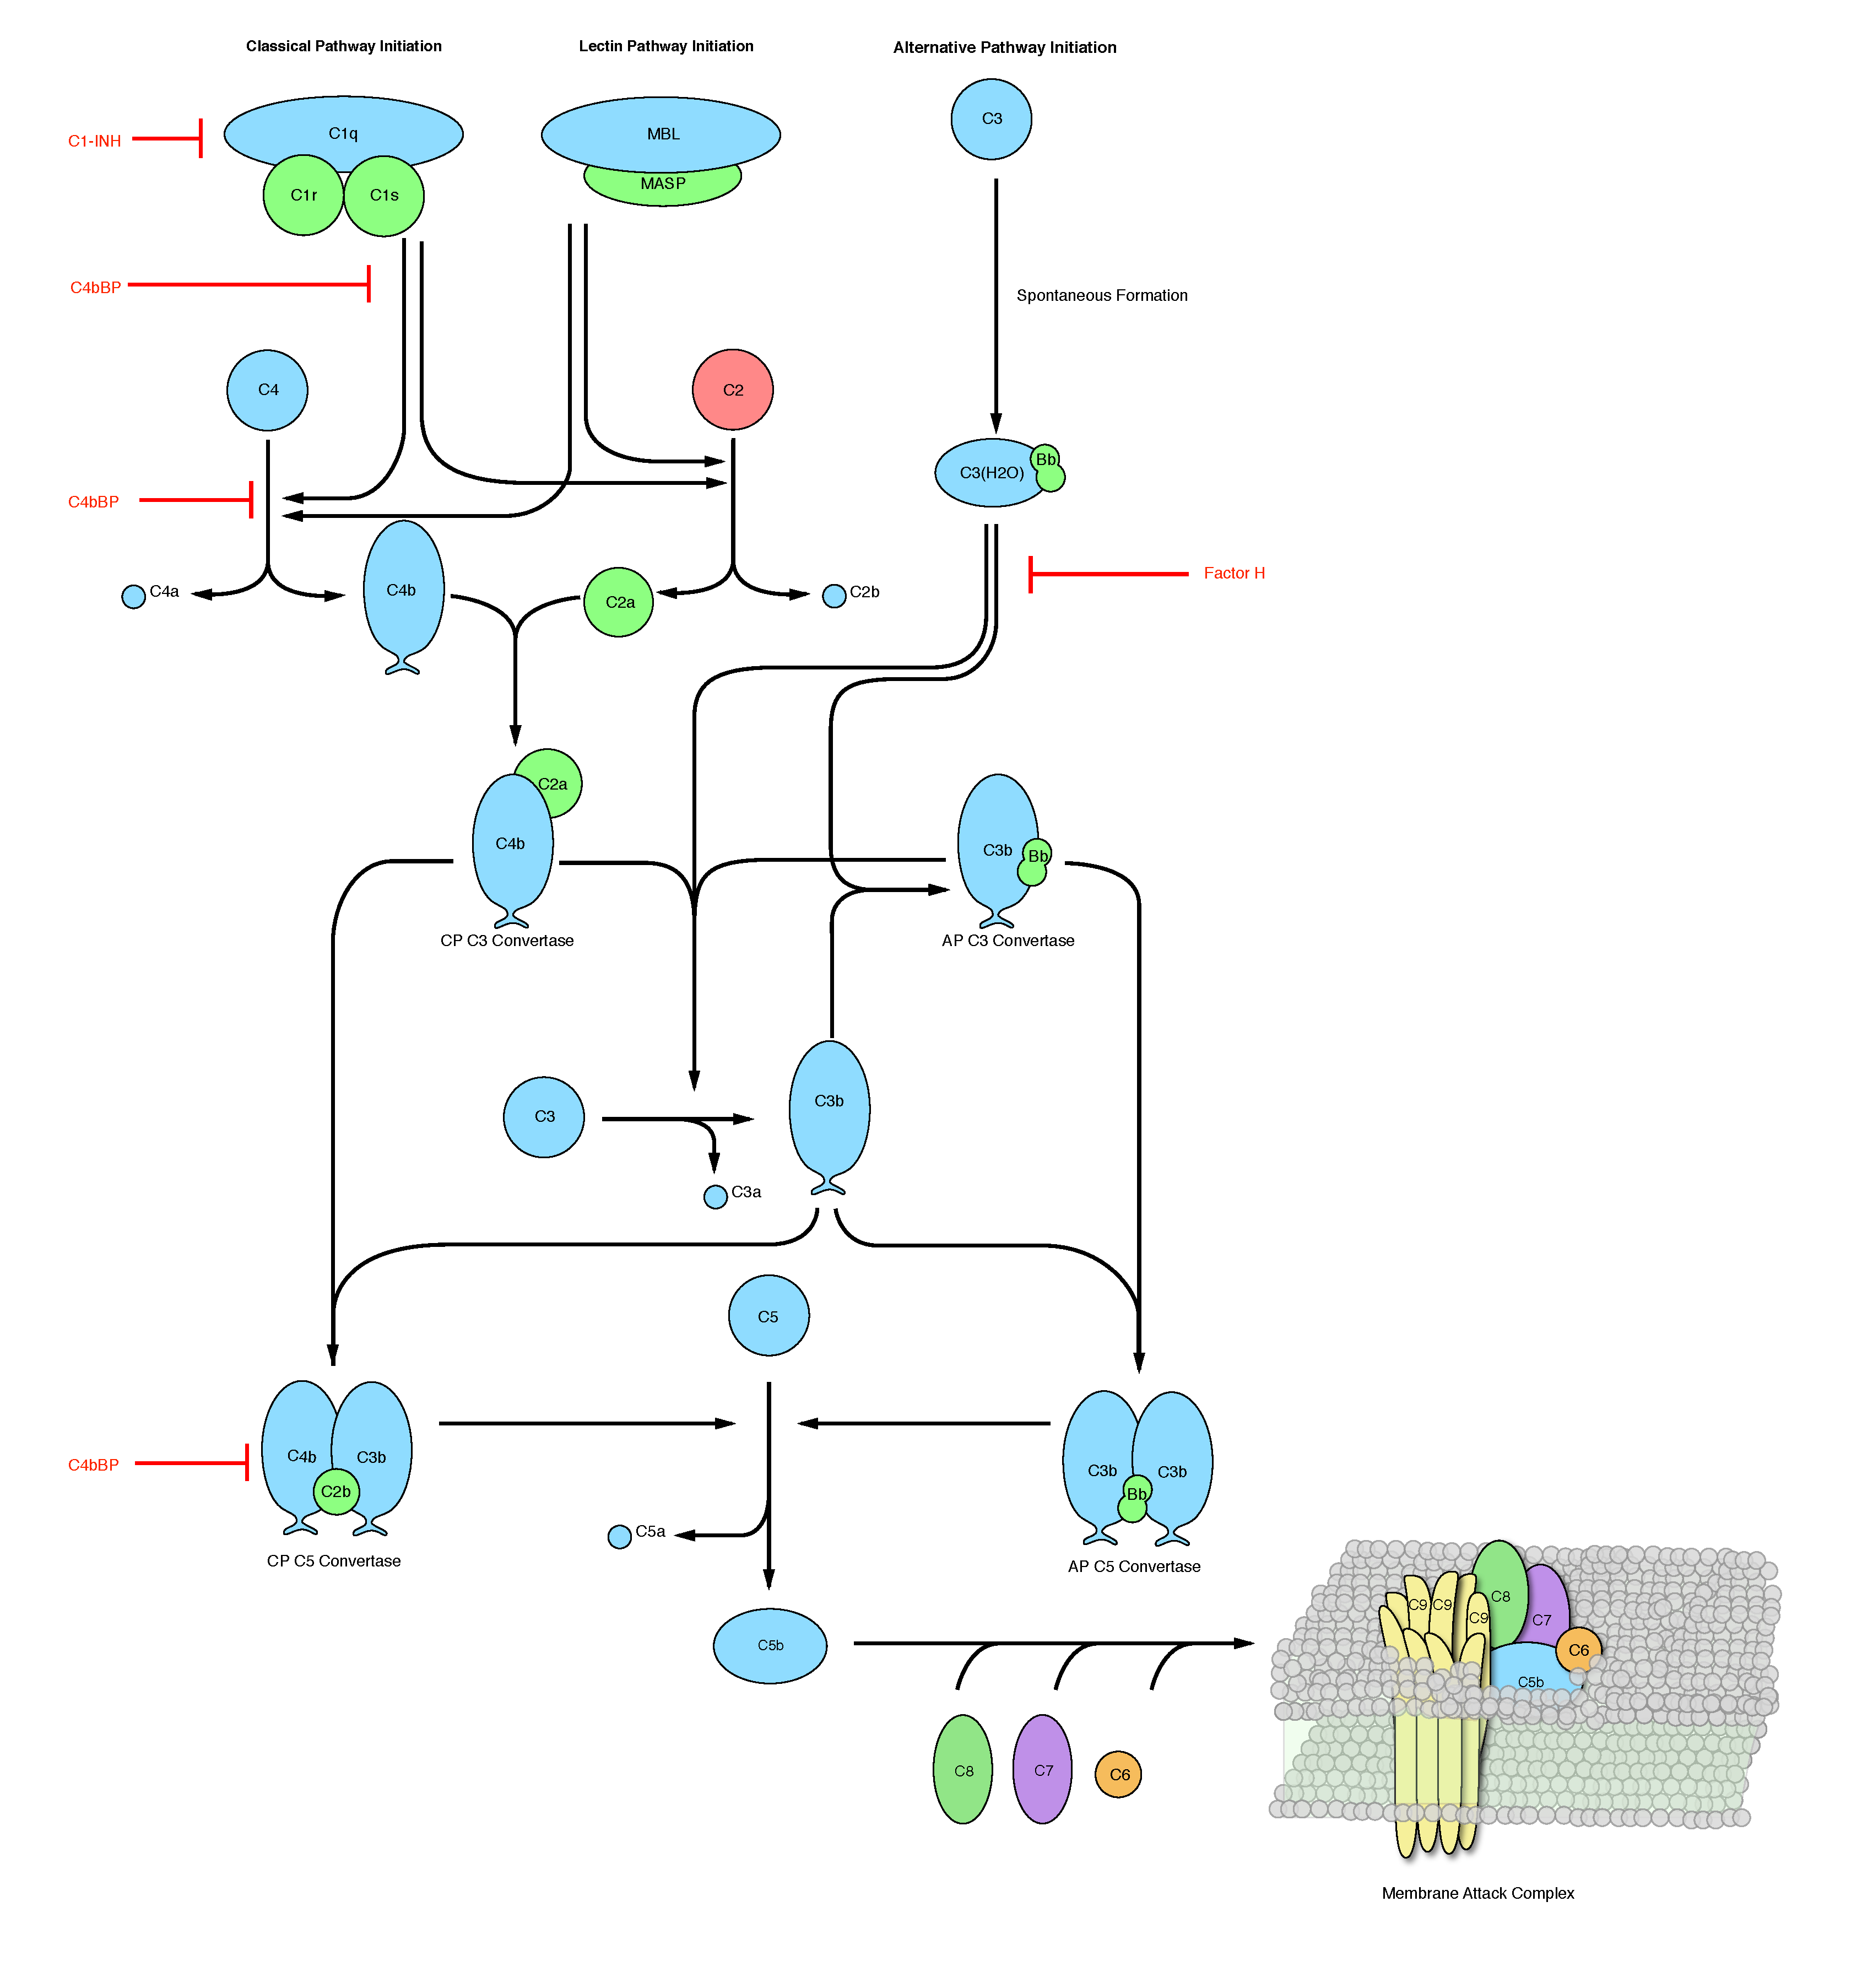
\includegraphics[width=1.0\textwidth]{./figs/ComplementSystemSchematic_v2.pdf}
\caption{Simplified schematic representation of the human complement system. The complement cascade is activated through any one, or more, of the three pathways: classical, lectin, and alternate pathway. The classical pathway is activated by the complex formation of $C1q$, $C1r$, and $C1s$ by the recogniztion of antibody:antigen complexes. Similarly, the lecin pathway is initiation by binding mannan-binding lectin to mannose on pathogen surfaces. Lastly, the alternative pathway is activated when a complement component is spontaneously bound to the surface of the pathogen of virus. The activation from the three pathways creates a cascades of reactions that forms the proteases, $C3$ Convertase that cleaves $C3$ into $C3a$, and $C3b$, the main effector molecule of the complement system. $C3b$ can find to a $C3$ convertase and form a $C5$ convertase that cleaves $C5$ into $C5a$, and $C5b$ that undergoes a series of reactions to form the membrane attach complex ($MAC$).}\label{fig-schematic}
\end{figure}

\begin{figure}[h]
\centering
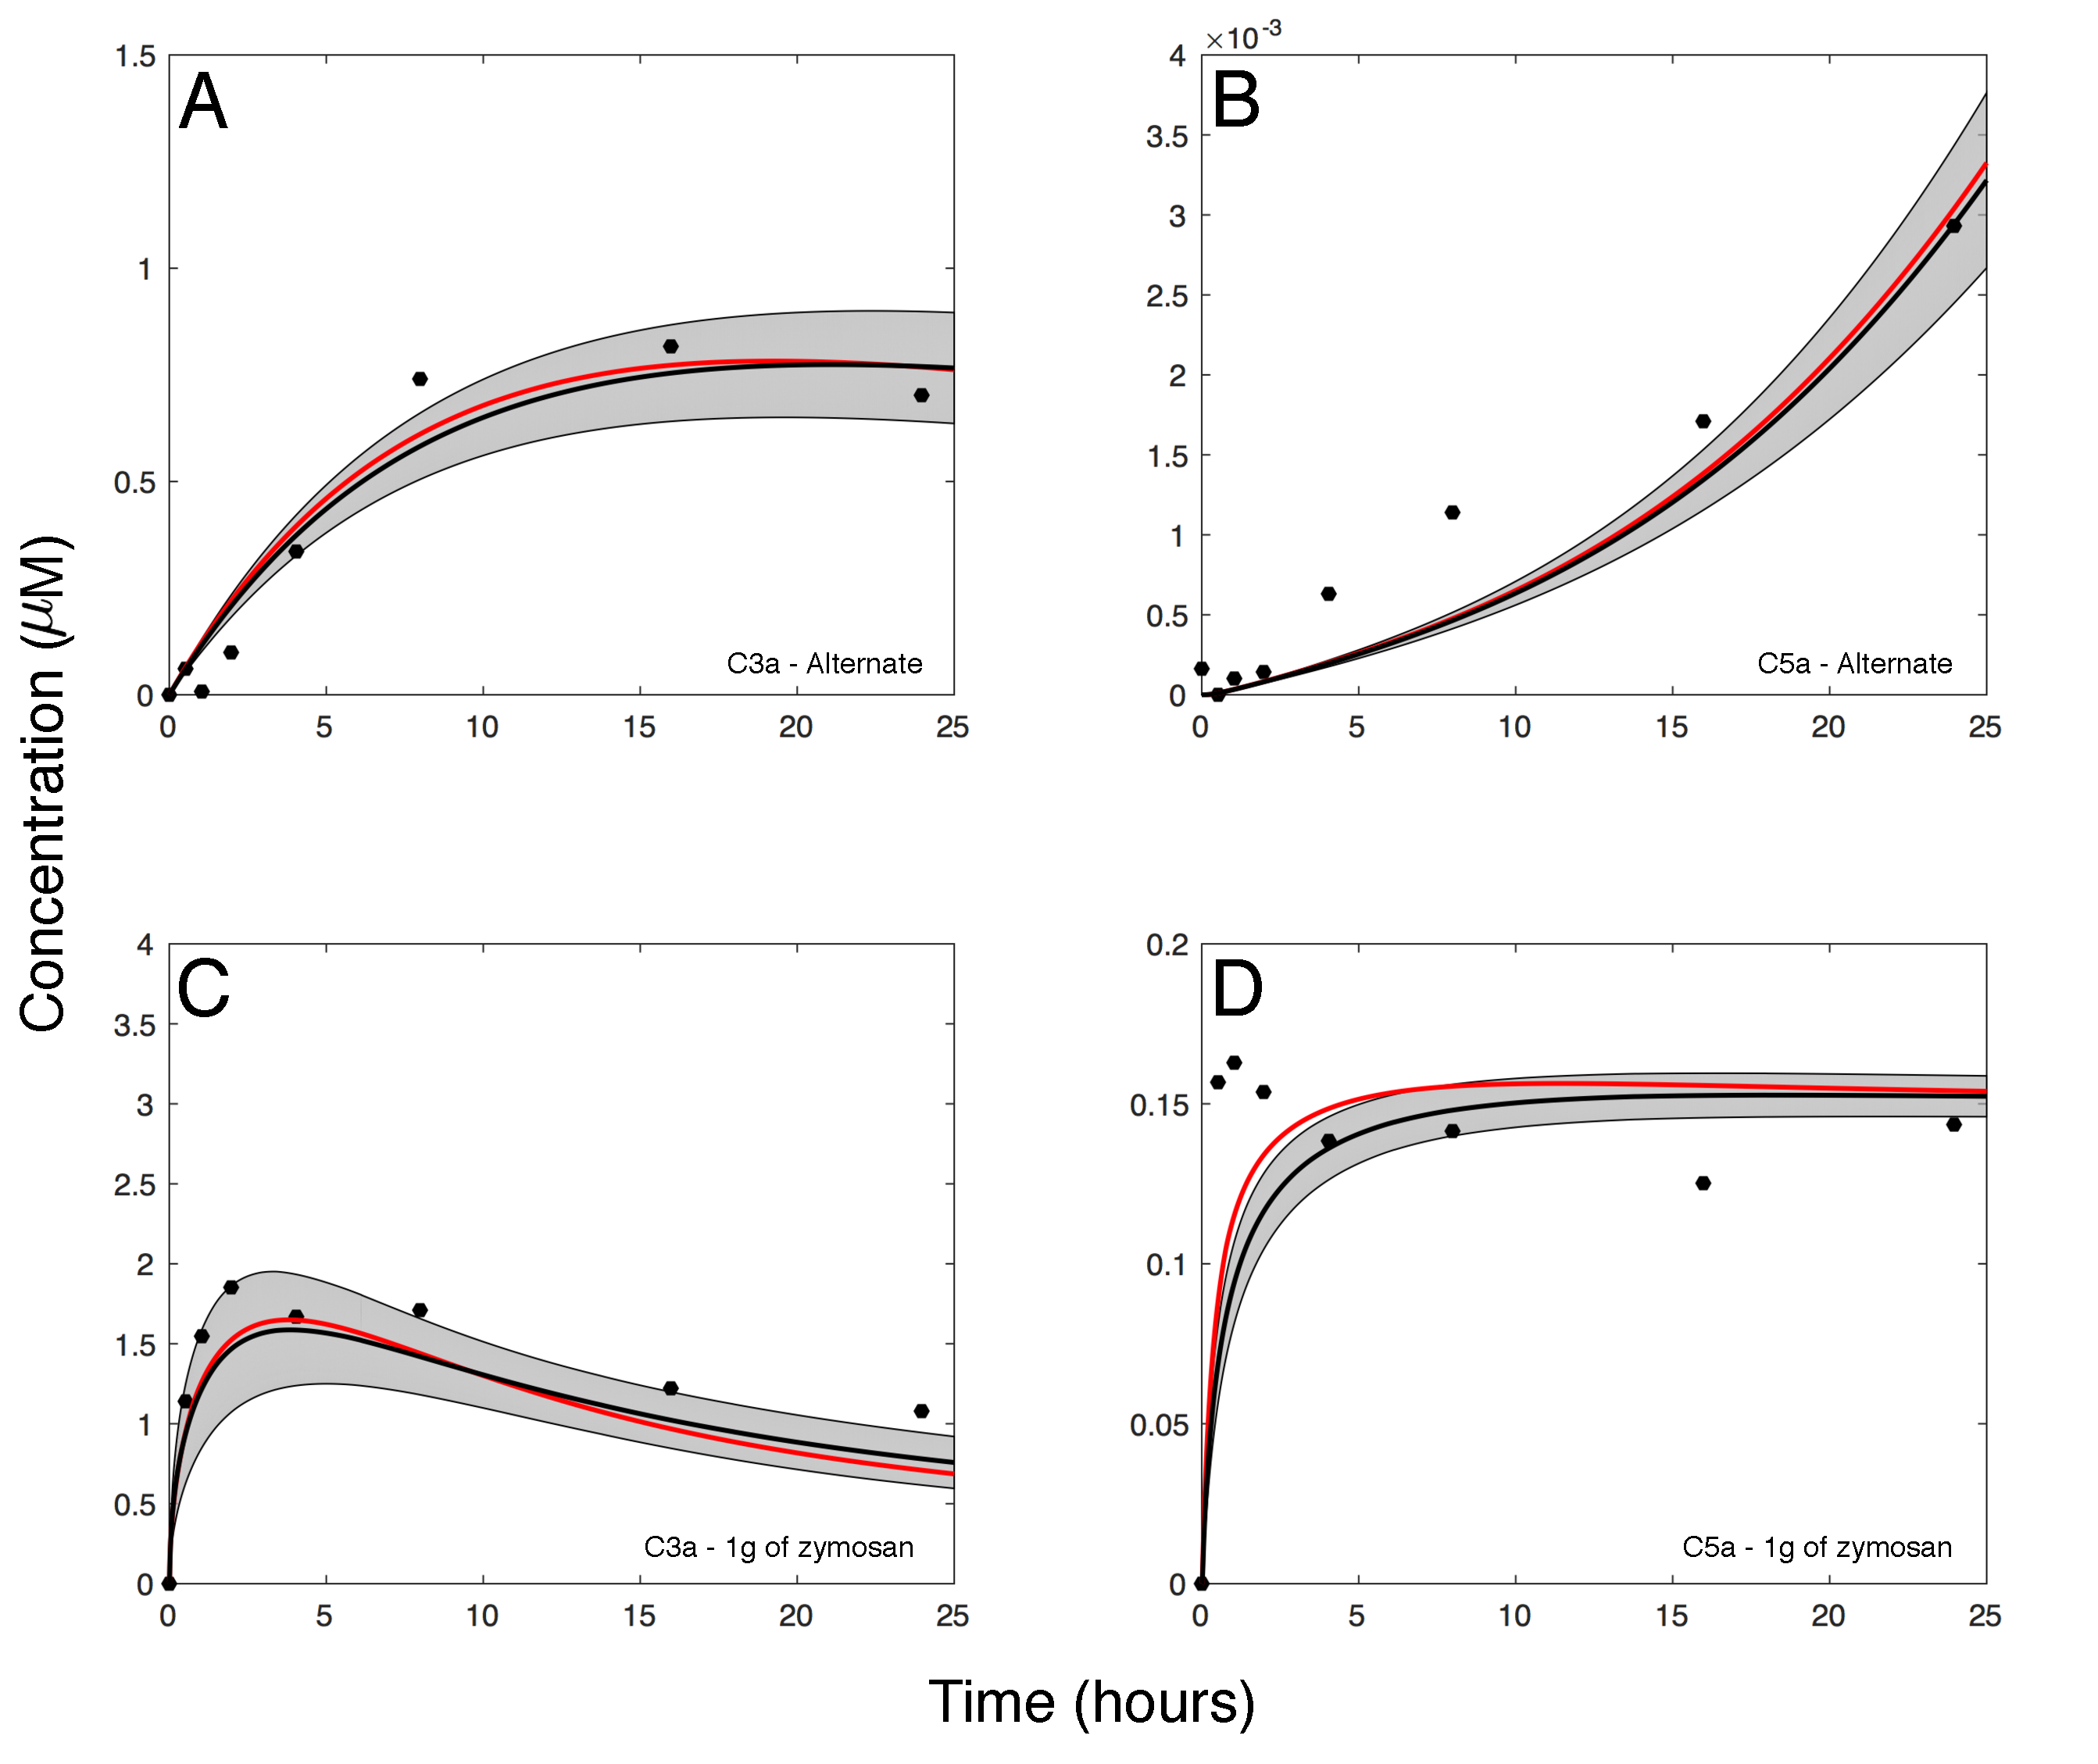
\includegraphics[width=1.0\textwidth]{./figs/Figure2_Fit.pdf}
\caption{Reduced order complement model training simulation for lectin and alternative pathway in presence of zymosan. Reduced order complement model parameters were estimated using dynamically dimensioned search (DDS) [Tolson and Shoemaker,2007,WRR] using the availability of zymosan as a function of lectin pathway initiation.  Only parameters that govern the behavior of alternative pathway were allowed to vary when zymosan was not present. Our model training was conducted in a hierarchal fashion where the alternate parameters were trained and then used and fixed in estimating the lectin parameters. The red line shows the best-fit parameter, the black lines denotes the simulated mean value of $C3a$ or $C5a$ for a 50 parameter set ensemble. The shaded region denotes the distribution of $C3a$ and $C5a$ of the ensemble.}\label{fig-fit}
\end{figure}

\begin{figure}[h]
\centering
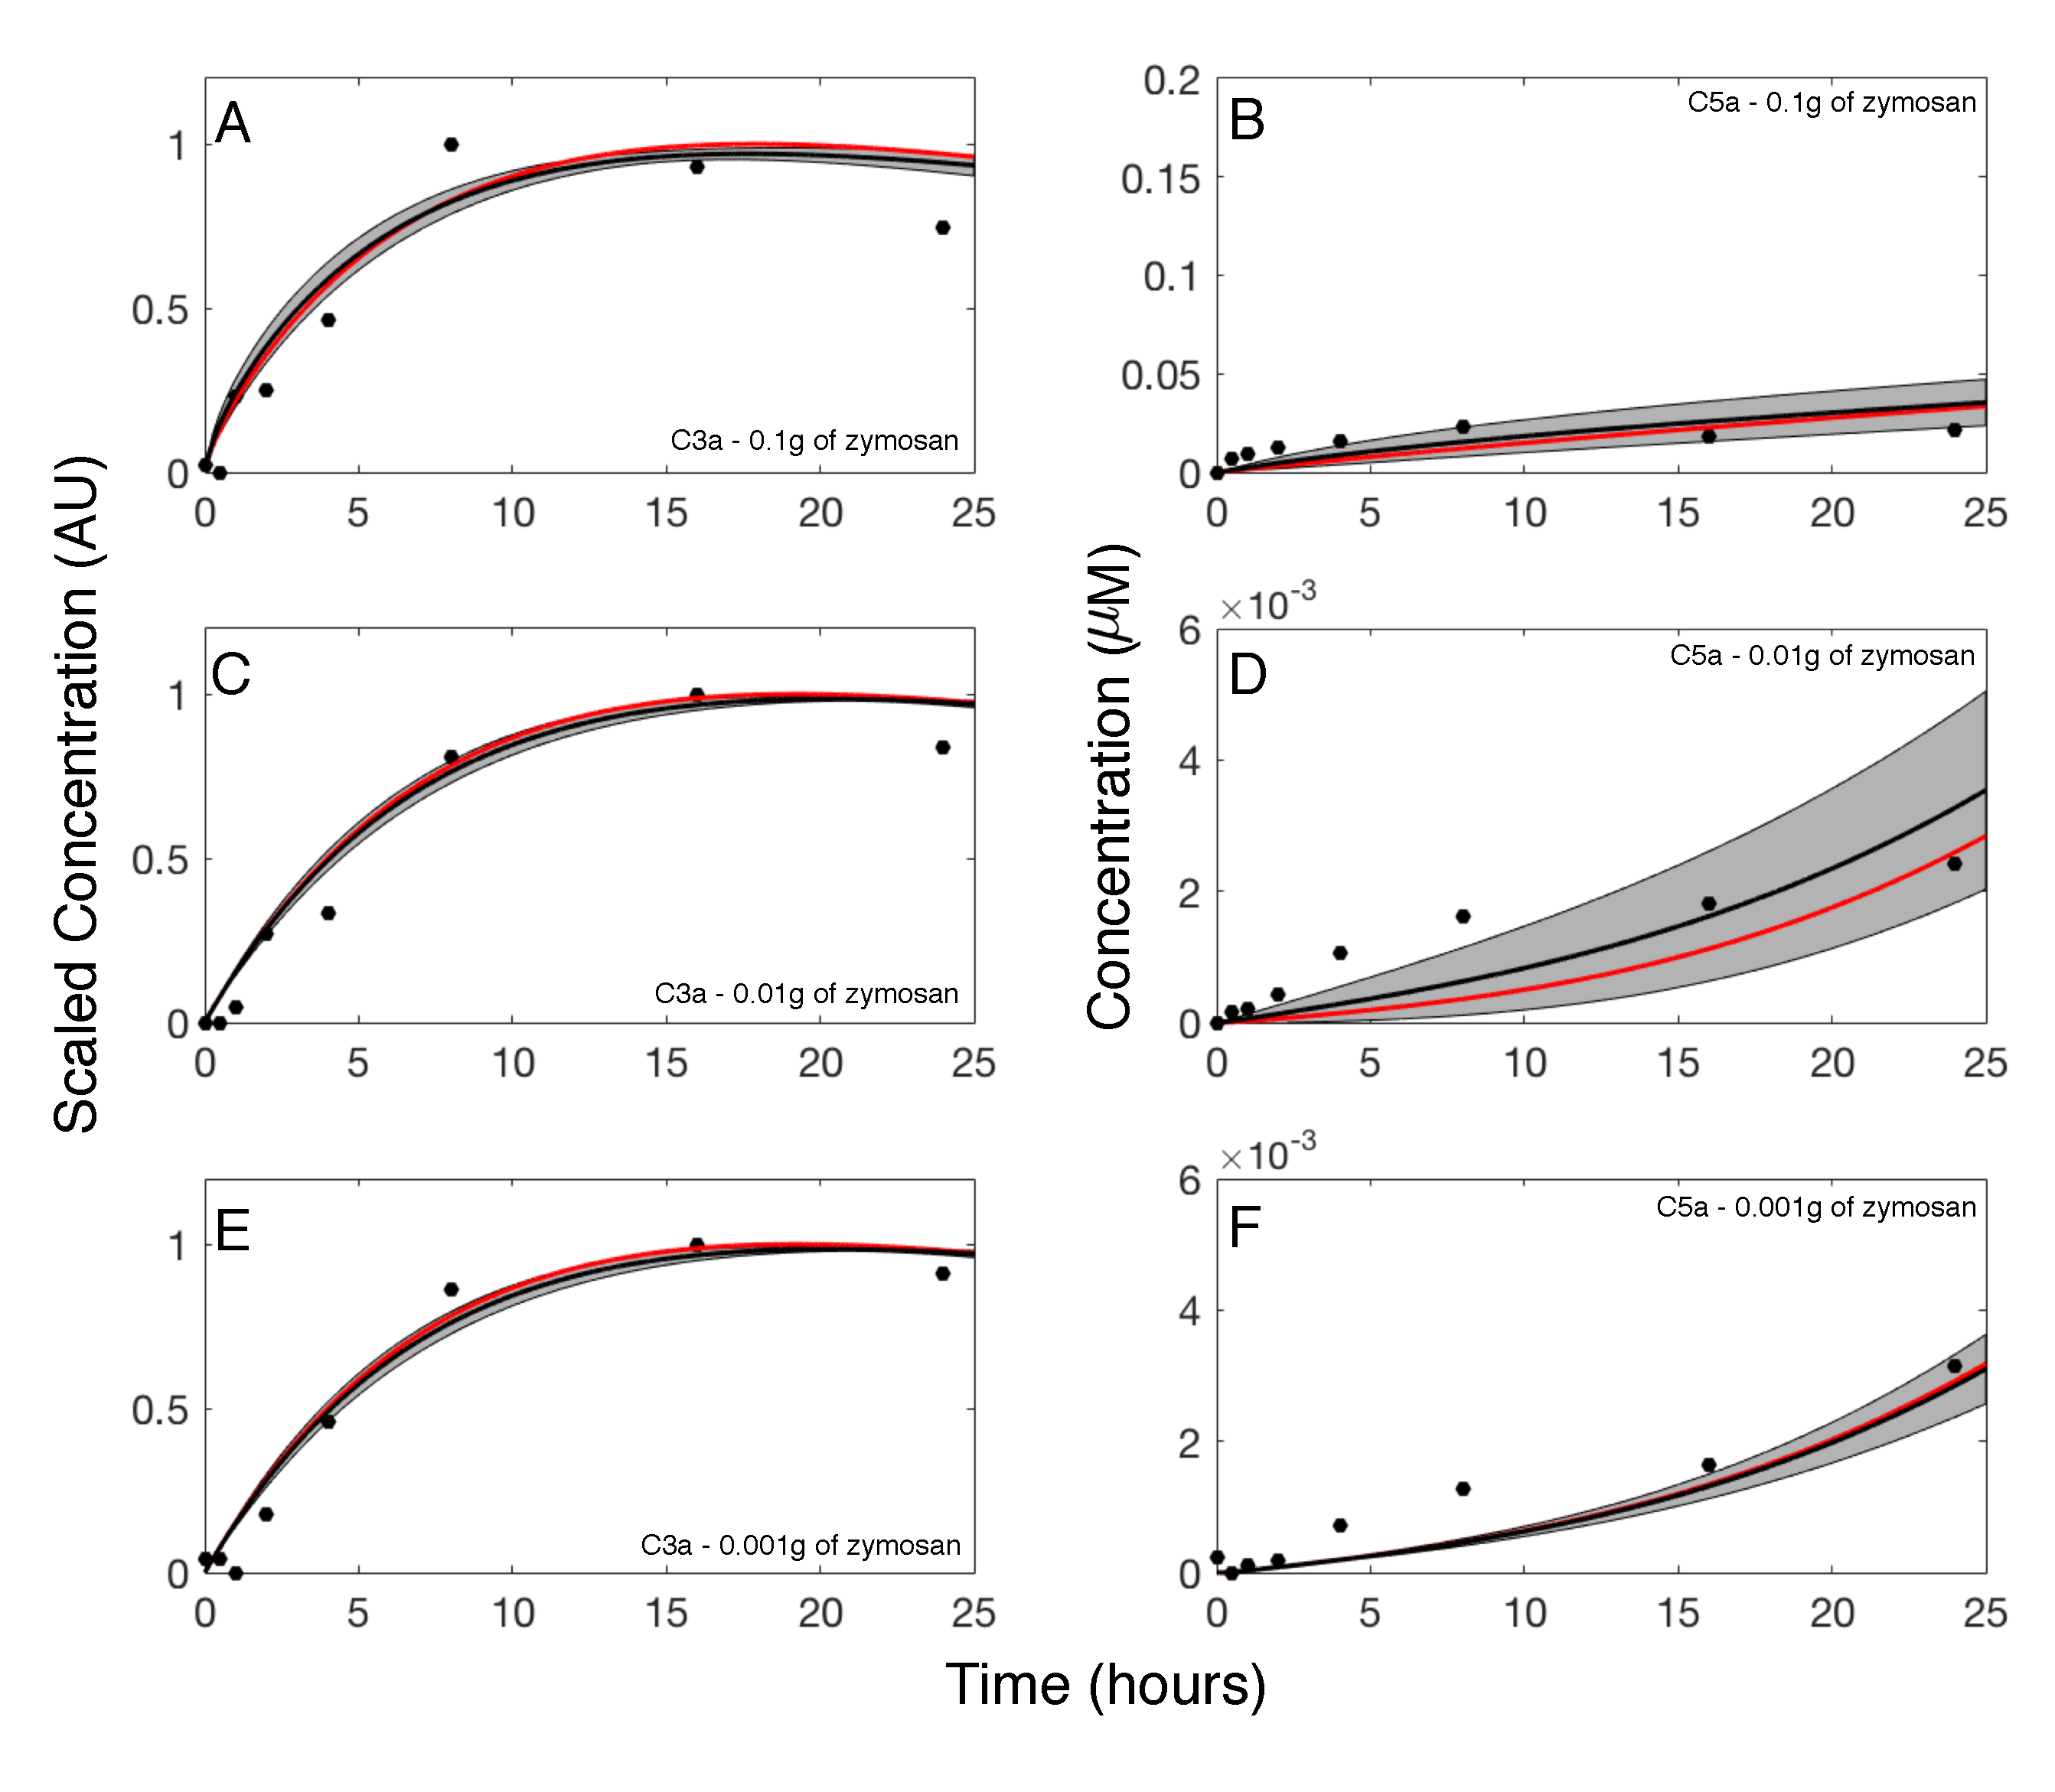
\includegraphics[width=1.0\textwidth]{./figs/Figure3_Predictions_2.pdf}
\caption{Reduced order complement model predictions of lectin and alternative pathway in presence of zymosan. (A-F) Simulation of complement dynamics in the presence of zymosan were conducted for a range of trigger values ($0.1$, $0.01$, and $0.001$ grams of zymosan). The time-course profiles of $C3a$ and $C5a$ under three different zymosan concentrations were simulated using 50 ensembles of trained parameter sets against experimental data of Shaw et al [REF].  The red curve represents the best fit parameter, grey shaded region denotes the prediction results from 50 ensembles of parameter sets, and the black curve is the mean of the ensemble. All complement protein and factor initial concentrations coincided with human serum levels unless otherwise noted.}\label{fig-prediction}
\end{figure}

\begin{figure}[h]
\centering
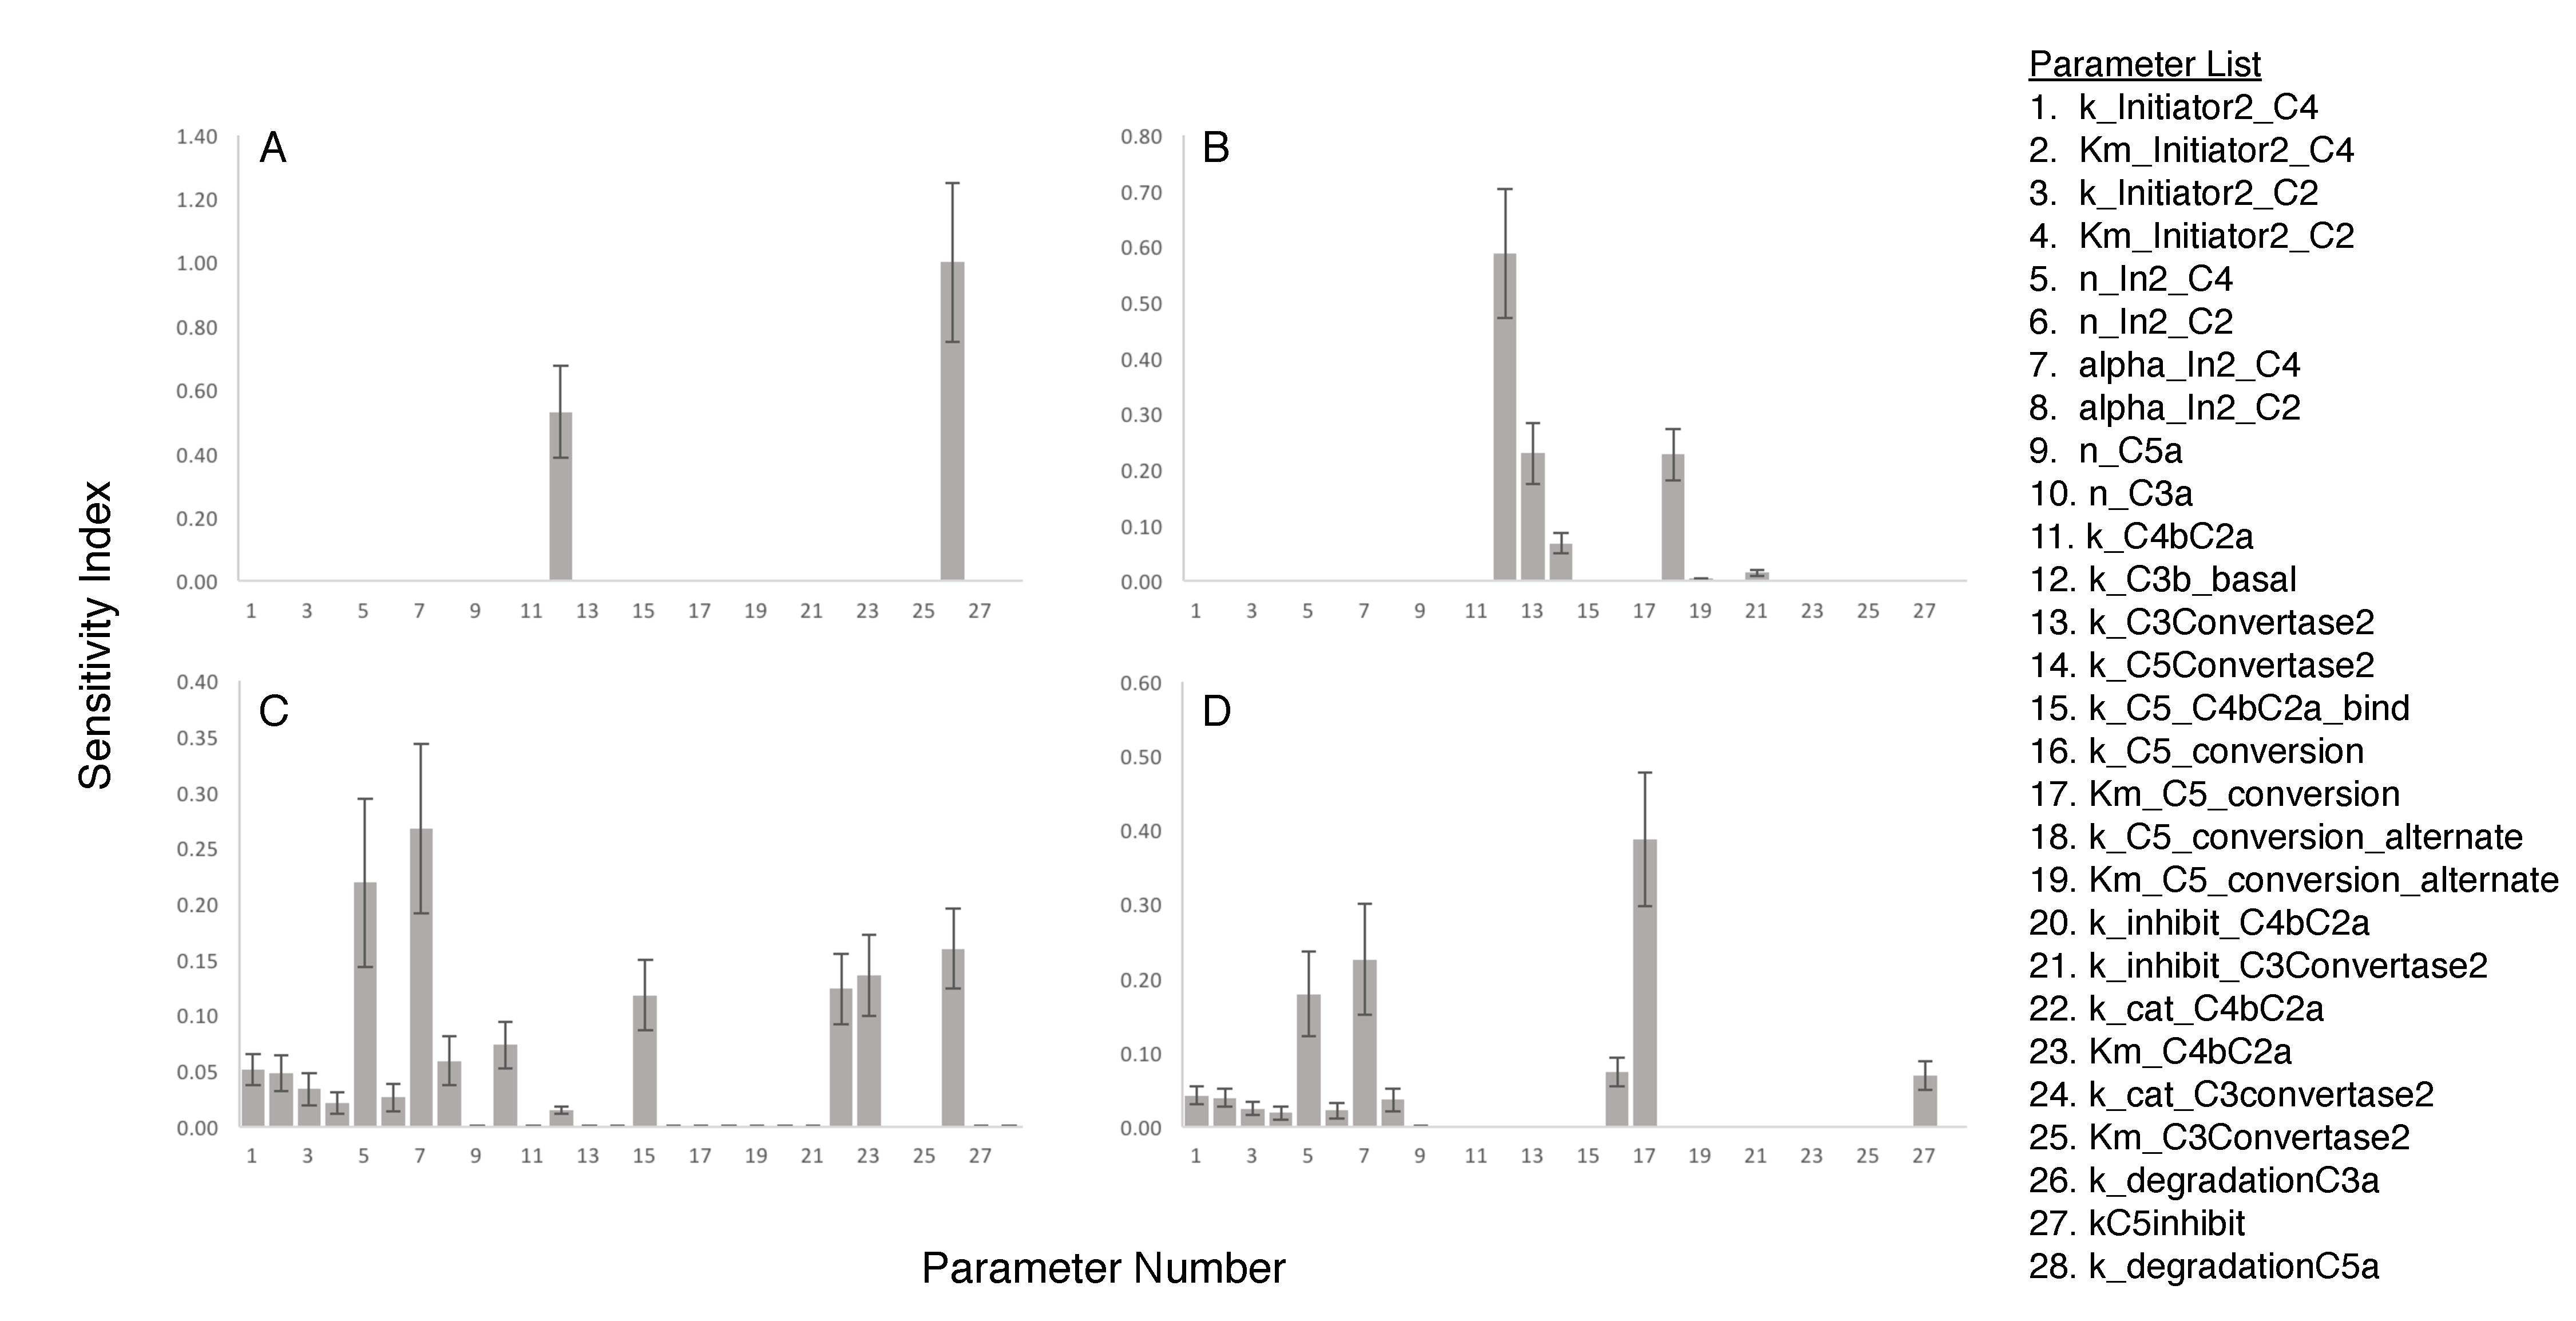
\includegraphics[width=1.0\textwidth]{./figs/Figure4_Sensitivity_Analysis_v2.pdf}
\caption{Sobol's sensitivity analysis of the reduced order complement model with respect to the modeling parameters.  Sensitivity analysis was conducted on the four cases we used to train our model: (A) C3a at 0 zymosan, (B) C5a 0 zymosan, (C) C3a 1 g zymosan, and (D) C5a $1$ g zymosan. The bars denote total sensitivity index which includes local contribution of each parameter and global sensitivity of significant pairwise interactions. The error bars are the 95 percent confidence interval. $k$ represents association rate, $km$ denote Michaelis-Menten saturation constants, and $alpha$ and $n$ refers to the exponentials of the control functions.}\label{fig-SA}
\end{figure}

\clearpage

% Supplemental figures -
% Set the S-
\renewcommand\thefigure{S\arabic{figure}}
\renewcommand\thetable{T\arabic{table}}
\renewcommand\thepage{S-\arabic{page}}
\renewcommand\theequation{S\arabic{equation}}

% Reset the counters -
\setcounter{equation}{0}
\setcounter{table}{0}
\setcounter{figure}{0}
\setcounter{page}{1}


\section*{Supplemental materials.}
\subsection*{Model equations.}
The reduced-order complement model consisted of 18 ordinary differential equations, 12 rate equations, and two control equations:
\begin{eqnarray}
	\frac{dx_{1}}{dt} & =& - r_{1}f_{1} \\ 								%C4
	\frac{dx_{2}}{dt} &=& - r_{2}f_{2} \\  								%C2
	\frac{dx_{3}}{dt} &=&  r_{1}f_{1} \\ 								%C4a
	\frac{dx_{4}}{dt} &=& r_{1}f_{1} - r_{6} \\ 					%C4b
	\frac{dx_{5}}{dt} & = & r_{2}f_{2} - r_{6} \\ 					%C2a
	\frac{dx_{6}}{dt} &=& r_{2}f_{2} \\ 								%C2b
	\frac{dx_{7}}{dt} &=& r_{3} - r_{4} - r_{5}\\ 				%C3
	\frac{dx_{8}}{dt} &=& r_{3}  + r_{4} + r_{5}  - k_{deg,c3a}*C3a \\		%C3a
	\frac{dx_{9}}{dt} &=& r_{3}  + r_{4} + r_{5}  -  r_{7} \\		%C3b
	\frac{dx_{10}}{dt} &=& r_{6} - r_{10} -  r_{8} \\			%CP C3C
	\frac{dx_{11}}{dt} &=& r_{7} - r_{11} -  r_{9} \\			%AP C3C
	\frac{dx_{12}}{dt} &=& r_{10} - r_{14} \\							%CP C5C
	\frac{dx_{13}}{dt} &=& r_{10}  \\											%AP C5C
	\frac{dx_{14}}{dt} &=& - r_{12} - r_{13} \\								%C5
	\frac{dx_{15}}{dt} &=&  r_{12} + r_{13} - k_{deg,c5a} \\					%C5a
	\frac{dx_{16}}{dt} &=& r_{12} + r_{13} \\								%C5b
	\frac{dx_{17}}{dt} &=& - r_{8} - r_{14} \\  				         %C4BP
	\frac{dx_{18}}{dt} &=& - r_{9} \\									%Factor H
\end{eqnarray}where the rate equations are given by:
\begin{eqnarray}
	r_{1} &=& \frac{k_{i1}(C4)}{(K_{1s} + C4)} \\
	r_{2} &=& \frac{k_{2}(C2)}{(K_{2s} + C2)} \\
	f_{1} &=& \frac{Zymo^{\eta_{1}}}{(Zymo^{\eta_{1}} + \alpha_{1}^{\eta_{1}})} \\
	f_{2} &=& \frac{Zymo^{\eta_{2}}}{(Zymo^{\eta_{2}} + \alpha_{2}^{\eta_{2}})} \\
	r_{3} &=& k_{3}(C3) \\
	r_{4} &=& \frac{k_{4}(C3C_{L})(C3^{\eta_{3})}}{(K_{4s}^{\eta_{3}} + C3^{\eta_{3}})}  \\
	r_{5} &=& \frac{k_{5}(C3C_{A})(C3)}{(K_{5s} + C3)} \\
	r_{6} &=& k_{6}(C4b)(C2a) \\
	r_{7} &=& k_{7}(C4b)(C2a) \\
	r_{8} &=& k_{8}(C3C_{L})(C4b)(C4BP) \\
	r_{9} &=& k_{9}(C3C_{A})(FactorH) \\
	r_{10} &=& k_{10}(C3C_{L})(C3b) \\
	r_{11} &=& k_{11}(C3C_{A})(C3b) \\
	r_{12} &=& \frac{k_{12}(C5C_{L})(C5^{\eta_{4}})}{(K_{12s}^{\eta_{4}} + C5^{\eta_{4}})} \\
	r_{13} &=& \frac{k_{13}(C5C_{A})(C5)}{(K_{13s} + C5)} \\
	r_{14} &=& k_{14}(C5C_{L})(C4BP)
\end{eqnarray}

% Supplemental figures go here ...
%\begin{figure}[ht]
%\centering
%\includegraphics[width=1.00\textwidth]{./figs/<Filename>.pdf}
%\caption{Captiontext goes here}
%}\label{fig:<label_name>}
%\end{figure}

\end{document}
